\section{Formato de mensajes}
Los mensajes enviados entre los nodos deben tener un formato compatible con las
redes CAN convencionales. Por ello el mensaje tiene un tamaño que varía desde
los 45 bits hasta los 109 bits (5 bytes hasta los 13 bytes), dependiendo de la cantidad de datos en el
\textit{Data Field}.

En la Figura \ref{fig:Data_Frame} se observa la el formato de Frame de datos de
los mensajes CANae.

\begin{figure}[h!]
 \centering
 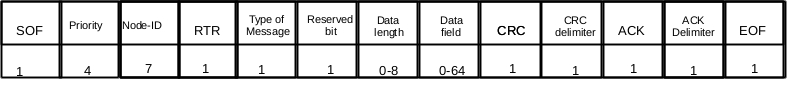
\includegraphics[scale=0.6]{images/Secciones/AppendixA/Data_Frame.jpg}
  \caption{Frame de datos CANae}
\label{fig:Data_Frame}
\end{figure}

Los campos del mensaje son los siguientes:

\begin{itemize}
\item Start of Frame (SOF) - 1 bit: Este bit marca el comienzo de un frame.
  Suele ser 0.
\item Priority - 4 bits: Este campo declara la prioridad del frame. 
\item Node-ID - 7 bits: El ID del Nodo origen.
\item Remote transmission request (RTR) - 1 bit: Bit dominante (0) para frames
  de datos o eventos, y bit recesivo (1) para frames remotos. Un frame remoto
  es un mensaje que es enviado en forma automática por algún sensor. Los frames
  remotos se utilizan para enviar telemetría por parte de los sensores y
  componentes.
\item Type of Message (TOM) - 1 bit: Bit dominante (0) si es un evento, y bit
  recesivo (1) para frames remotos.
\item Bit reservado - 1 bit: Este bit está reservado para futuras aplicaciones.
  En esta versión debe ser un bit dominante (0).
\item Data length - 6 bits: Cantidad de bytes del campo de datos.
\item Data field - 0-64 bits (0-8 bytes): Datos.
\item CRC - 15 bits: Cyclic redundancy check.
\item CRC delimier - 1 bit: Debe ser recesivo (1).
\item ACK - 1 bit: El transmisor debe poner este bit en recesivo (1), y el
  receptor puede responder este bit con un bit dominante (0).
\item ACK delimiter - 1 bit: Debe ser recesivo (1).
\item End-of-Frame (EOF) - 7 bits: Final del frame de datos.
\end{itemize}

El \textit{Data Field} tiene el siguiente formato: el primer byte siempre es
el ID de la función, evento y/o comando. Esto significa que es posible definir
un número de $2^8 = 256$ funciones, eventos y comandos diferentes.

Los siguientes bytes (del 1 al 63) son argumentos de las funciones o datos.

Debe entenderse que esto no es mandatorio, ya que se pueden definir ID de
dos o más bytes reduciendo la cantidad de datos.

\subsection{Start of Frame}
Este bit marca el comienzo de un mensaje CANae. Este es simplemente un bit
dominante (0). Para que un dispositivo pueda enviar mensajes, el bus debe estar
en estado IDLE.

\subsection{Priority}
Este campo indica la prioridad del mensaje. La prioridad está compuesta por 4
bits, por lo tanto acepta una cantidad de $2^4$ niveles de prioridad. La
prioridad máxima es 0000, mientras que la mínima es 1111.

\begin{table}[h!]
  \centering
  \caption{Prioridades de mensajes}
  \label{tab:prorities}

  \begin{tabular}{|l|l|l}
    \cline{1-2}
    Priority Field & Prioridad & \\ \cline{1-2}
    0000 & 0 & Alta prioridad \\ \cline{1-2}
    0001 & 1 & ... \\ \cline{1-2}
    ... & ... & ... \\ \cline{1-2}
    1111 & 15 & Baja prioridad \\ \cline{1-2}
  \end{tabular}
  
\end{table}

\subsection{Node-ID}
Este indica el ID del nodo que envía el mensaje. Este campo está compuesto por 7
bits, lo cual posibilita la existencia de hasta $2^7 = 128 $ nodos conectados
a la red.

\subsection{Remote transmission request (RTR)}
Este permite diferenciar un frame que sea remoto o un mensaje ``normal''. Un
frame remoto es aquel que se utiliza para enviar telemetría. Comúnmente es
enviado por sensores y componentes. El bit dominante (0) indica que es un frame
``normal'' (contiene un mensaje o un evento), un bit recesivo (1) indica que es
un frame remoto.

\subsection{Type of Message (TOM)}
Este campo es de 1 bit. Diferencia frames de mensajes con frames de eventos.
Si el bit es dominante (0) significa que se trata de un frame de evento. Si el
bit es recesivo (1) significa que se trata de un frame de mensaje. Debe tenerse
en cuenta que si el bit RTR es recesivo (1), el bit TOM obligatoriamente debe
ser recesivo (1) indicando que el frame trae consigo un mensaje con los datos de
telemetría.

\subsection{Bit reservado}
Bit reservado.

\subsection{Data length}
Indica el tamaño del campo de datos (\textit{Data Field}). Este campo esta
compuesto por 6 bits. 

\subsection{Data field}
En este campo se agregan los datos del mensaje. El primer byte del
\textit{Data Field} es el código de la función y/o evento. Los bytes
subsiguientes pueden ser los argumentos y/o datos de la función o evento que se
está enviando en el frame. Se pueden enviar solo una función a la vez, y hasta 7
datos o argumentos. 

\subsection{CRC}
En este campo se almacena el CRC del frame. Para calcular el CRC se utiliza el
polinomio de CAN.

$$x^{15} + x^{14} + x^{10} + x^{8} + x^7 + x^4 + x^3 + 1$$

El algoritmo para resolver el CRC se muestra en \ref{cod:CRC}.

\lstset{language=C,caption={Función para resolver CRC},label=cod:CRC}
\begin{lstlisting}
  uint16_t crc_c(uint8_t data, uint16_t crc){
  uint8_t i;

  crc ^= (uint16_t)data << 7;
  for (i = 0; i < 8; i++){
    crc <<= 1;
    if(crc & 0x8000){
      crc ^= 0xc599;
    }
  }
  return crc & 0x7fff;
}
\end{lstlisting}

\subsection{CRC delimiter}
Este es un bit recesivo (1) para indicar que el CRC Field finalizó.

\subsection{ACK}
El transmisor debe poner este bit en recesivo (1), y el receptor puede responder
el mensaje colocando este bit en dominante(0).

\subsection{ACK delimiter}
Este bit indica el final del ACK. Este es un bit recesivo (1).

\subsection{End-of-Frame (EOF)}
Indica el final del frame de datos. Debe ser recesivo, es decir, los 7 bits en
1.
